% This is a template file for submitting your homework in math 301. 

\documentclass[letter]{article} %This tells the LaTeX compiler what type of document we are creating

%The next few lines are packages that we load. Geometry allows us to change the margins and other page properties. The amsmath and amssymb packages give us access to common math symbols. 

\usepackage[margin=1in]{geometry}
\usepackage{amsmath}
\usepackage{amssymb}
\usepackage{ifthen}
\usepackage{fancyhdr}
\usepackage{color}
\usepackage[fleqn]{nccmath}
\usepackage{graphicx}
%\graphicspath{ {C:/Users/joh10/Desktop/FSU/CompStat1/Assignments/hw6/} }

%I would like to have space to write comments on your work.  The linespread command below will add extra space to your document.
\linespread{1.5}
 
\pagestyle{fancy}
\rhead{\ifthenelse{\value{page}=1}{\noindent Homework 4 - TISP \hfill Kyle Shaw, Thomas Johansen \\
Oct. 3, 2017 \hfill STA 5635}{Shaw/Johansen}}

\rfoot{\thepage}
\renewcommand{\headrulewidth}{0pt}
\renewcommand{\footrulewidth}{0pt}
\cfoot{}

%We are now ready to start our document.  The next line tells the computer to start creating the PDF. 
\begin{document}
\setlength{\headsep}{0.5 in}
%The section* command below creates an unnumbered section.  If you remove the *, you'll see it numbers the section as section 1. 

We performed classification on three datasets using logistic regression, employing a Thresholding-based Iterative Selection Procedure (TISP) for feature selection. The three datasets included in the report are Gisette, Arcene, and Madelon. The plots below show the misclassification error vs. the number of features included in the model for the training and testing sets for each dataset.  A summary table is also included showing the errors and lambda values for each subset of features.

\section*{Gisette}
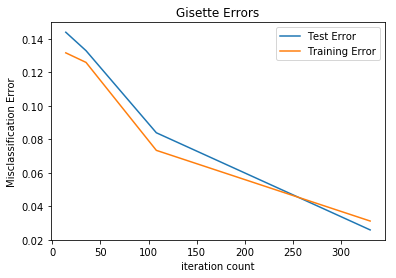
\includegraphics[scale=0.8]{gisette}

\section*{Arcene}
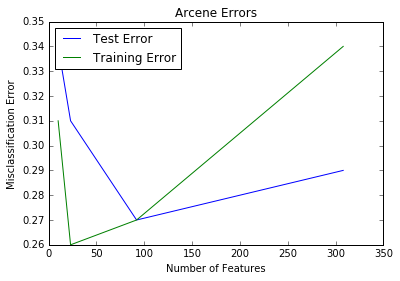
\includegraphics[scale=0.8]{arcene}

\clearpage
\newgeometry{top=1in, bottom=1in}

\section*{Madelon}
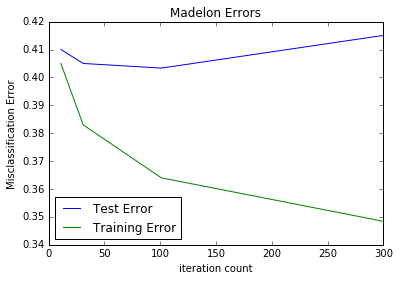
\includegraphics[scale=0.8]{madelon}

\section*{Summary of Misclassification Error}
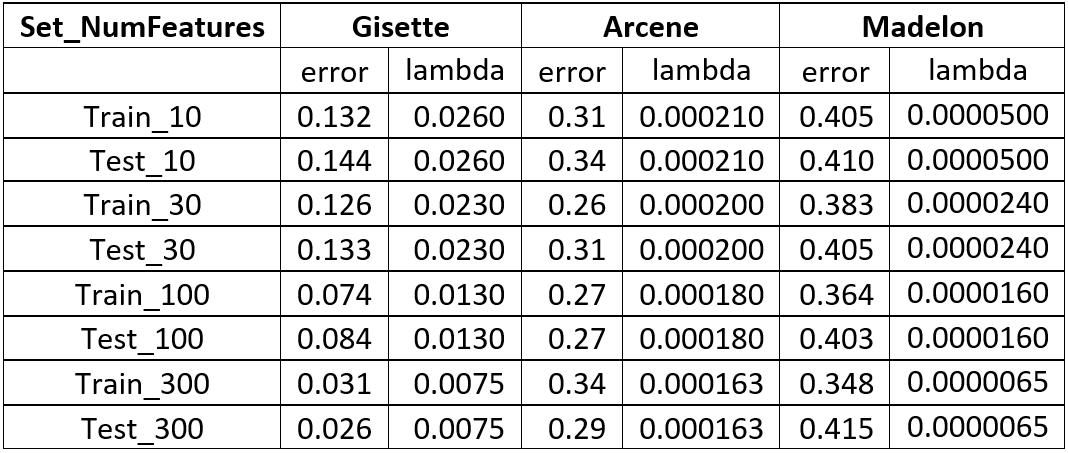
\includegraphics[scale=0.7]{table}

\clearpage

\section*{Some of the code}
\begin{verbatim}
from import_data import import_data
from sklearn import preprocessing
import matplotlib.pyplot as plt
import numpy as np

def updateWeights(X,X1,Y,w, Ncol,Nrow, learningRate, lam, thresh):
    tmp = w[1:Ncol]
    product = np.dot(X,tmp)
    shiftedValue = w[0] + product
    expValue = np.exp(shiftedValue)
    ratio = expValue / (1 + expValue)
    error = Y - ratio
    dLnew = np.dot(np.transpose(X1),error)
    w = w + learningRate * (-lam*w + dLnew/Nrow)
    w = (w) * (abs(w) >= thresh)
    #print(sum())
    return w

def Test(w, X, Y):
    #nomralize data
    X = preprocessing.scale(X)
    #Add column of 1s
    X = np.array(np.c_[np.ones((len(X), 1)), np.matrix(X)])
    Y = [0 if y <= 0 else 1 for y in np.array(Y)]
    wx = 1/(1+np.exp(-1 * np.dot(X, w)))
    Ypredict = [0 if x < .5 else 1 for x in wx]
    results = np.array(Y) - np.array(Ypredict)
    return sum(abs(results))/len(Y)
    
def Plot(x,y1,y2,title,legendLoc = 1):
    plt.title(title)
    plt.plot(x,y1,label = 'Test Error')
    plt.plot(x,y2,label = 'Training Error')
    plt.legend(loc = legendLoc)
    plt.xlabel('Number of Features')
    plt.ylabel('Misclassification Error')
    plt.show()
    
def TrainWeights(X,Y,Xtest,Ytest,k, learnRate = .01, thresh = .001):
    X = preprocessing.scale(X)
    Y = [0 if y <= 0 else 1 for y in np.array(Y)]
    X1 = np.array(np.c_[np.ones((len(X), 1)), np.matrix(X)])
    #initialize variables
    Nrow = len(X)
    Ncol = len(X1[0])
    learningRate = learnRate
    lam = .001    
    w = np.array([0]*(Ncol))    
    y1 = []
    y2 = []
    for i in range(k):
        w = updateWeights(X,X1,Y,w, Ncol,Nrow, learningRate, lam, thresh)
        y1.append(Test(w,Xtest, Ytest))
        y2.append(Test(w,X,Y))
        if(i%10 == 0):
            print(sum(abs(w) >= thresh))        
    return y1,y2

#Gisette Data
##Read in the Data
X, Y, Xtest, Ytest = import_data('gisette', 'gisette_train.data', 'gisette_valid.data',
	'gisette_train.labels', 'gisette_valid.labels', head = None)
X.drop(X.columns[len(X.columns)-1], axis=1, inplace=True)
Xtest.drop(Xtest.columns[len(Xtest.columns)-1], axis=1, inplace=True)  

niter = 100
y1, y2 = TrainWeights(X,Y,Xtest,Ytest,niter,.1, .02)
# guess and check to get the numbers for the plot below
Plot([11, 31, 101, 299], [.144, .133, .084, .026], [.1317, .126, .0735, .0313], 
	'Gisette Errors', 3)
min_table['Gisette'] = [min(y1), min(y2)]
\end{verbatim}

\clearpage
\newgeometry{top=1in, bottom=1in, left=0.5in}
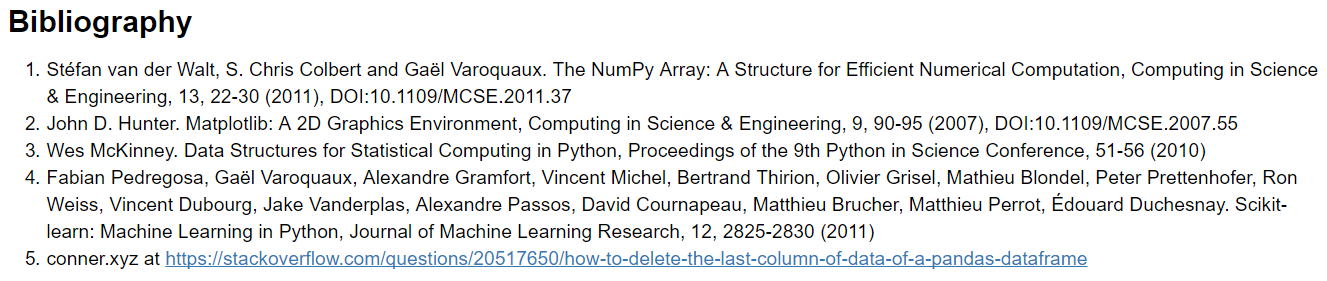
\includegraphics[scale=0.68]{bib}


\end{document}














